\documentclass[12pt]{article}
\usepackage{amsmath,amssymb,graphicx,rotating,fancyvrb}
\usepackage[margin=2.8cm]{geometry}
%\newcommand{\sw}[1]{\begin{sideways}#1\end{sideways}}
\newcommand{\sw}[1]{\footnotesize{}#1}
\newcommand{\cmark}{\checkmark}
\newcommand{\xmark}{$\times$}
\title{Dryer21, a Bitcoin Anonymizer Service}
\author{Adam Suhl, Danny Ben-David, Peter Schmidt-Nielsen}
\begin{document}
\maketitle
\begin{abstract}
Bitcoin transactions are stored in the blockchain (effectively a public ledger), which makes Bitcoin merely pseudonymous, rather than fully anonymous.
The canonical solution to this problem is a \emph{mixer} that receives ``dirty'' Bitcoins from many users, routes them all through a single mixing address, and dispenses them back out to new ``clean'' output addresses in a random order, or at random times.
We provide Dryer21, an implementation of such a mixing service that gives unusually strong privacy guarantees.
Specifically, through the use of Chaum's blind signing protocol we guarantee that no one -- not even the administrators of the Dryer21 service -- can link which dirty input addresses correspond to which clean output addresses.
Dryer21 is implemented as a highly privilege separated Python application, which is run as a Tor hidden service.
Additionally, a client script for using this service is provided.
\end{abstract}

\section{Overview}
As with any Bitcoin mixing service, Dryer21 aggregates payments from a large set of clients through a single mixing address, and issues payments back out in a randomized fashion.
If the payout schedule is appropriately designed then even an adversary with complete access to the transaction record cannot reliably link payments into and out of the mixing service.
%Many different payout schedules are possible, each with its own corresponding anonymity/usability tradeoff.

Our scheme opts for simplicity by using a bond selling and redeeming mechanism.
Users purchase bonds from our server, and then are free to redeem them at a date and time of their choice.
These bonds are of a fixed denomination (currently 100 mBTC, or about \$35), to prevent payments from being linked by their exact size.
However, the most exciting feature of Dryer21 is that these bonds are issued using blind signatures, which results in the server being provably unable to link input and output addresses.
This feature will be discussed in more detail shortly.

\begin{figure}[ht]
\begin{center}
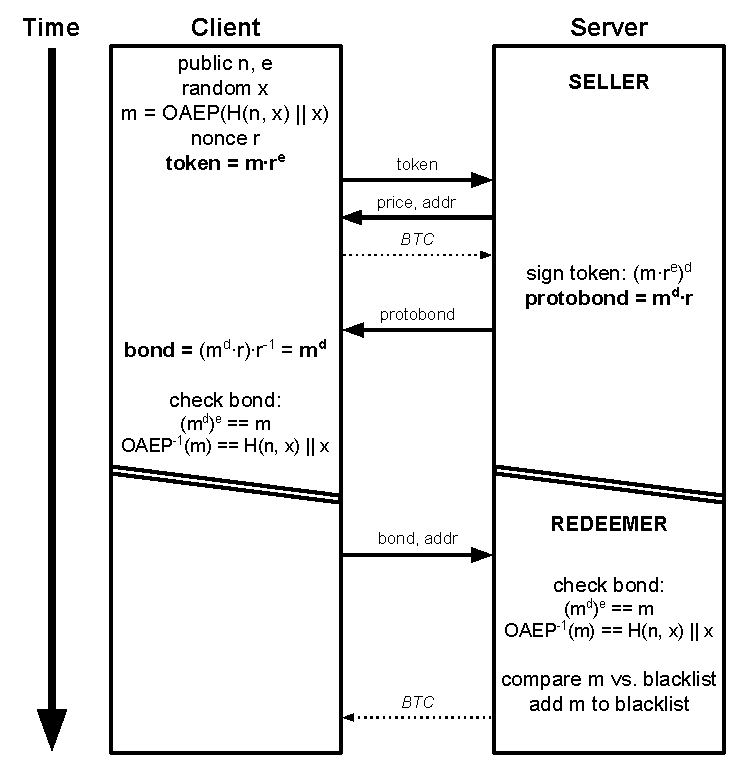
\includegraphics[width=10cm]{dryer21-crypto.pdf}
\end{center}
\caption{The entirety of the Dryer21 protocol in a nutshell.\label{over}}
\end{figure}

The Dryer21 server has a publicized bond signing RSA key with public exponent $e$ and private exponent $d$.
Any message fitting a particular exact format signed under this key will be considered a valid bond that the server is obligated to make good on.
The protocol for buying bonds proceeds as follows, and is summarized in figure \ref{over}.
\begin{enumerate}
\item The client generates a randomized unsigned bond $m$ fitting the special bond format, and blinds it by multiplying by $r^e$ for a randomly chosen nonce $r$.
This produces the \emph{token} $m r^e$ shown in figure \ref{over}, which is sent to the server.
\item The server stores this token, and replies with a price quote and Bitcoin address for the client to pay to.
\item Upon receiving payment from the client, the server signs the token to produce the \emph{protobond} $(m r^e)^d = m^d r$, and sends it back to the client.
\item Finally, the client multiplies the protobond by $r^{-1}$, yielding $(m^d r) r^{-1} = m^d$, which is a valid bond.
\end{enumerate}
Observe that the server only ever learns the protobond $m^d r$, which is the actual bond multiplied by a random group element $r$ known only to the client.
Therefore, the server learns absolutely nothing about the bond $m^d$.
This is the key insight that gives us our privacy guarantees.
Naturally, there are numerous additional messy details, such as correctly using OAEP in the right places to break the homomorphic structure of RSA, but these details can be found in any cryptography text covering blind signatures, and are unimportant to this high-level overview.

At some later date the client redeems his or her blinded bond by simply sending it to the server along with a requested payout address.
The server encrypts the blinded bond, and verifies that it is of the prescribed format.
At this point the server blacklists the bond, permanently marking it as used up, and issues the requested payment from the main mixing wallet.

Because the client connects via separate Tor circuits for buying and redeeming the bond, his or her payment and payout addresses are completely unlinkable.
Further, because the bond was blindly signed, they're not even linkable by the server itself!

\section{Privilege Separation}
The main obstacle in developing Dryer21 was writing a server that automatically performs Bitcoin transactions to fulfill bonds in a secure way.
To do this, we developed a simple framework for privilege separating a server via chrooted processes that communicate via RPC, then designed the entire server within this framework.
The access control policies for the entire server are defined through a series of declarations like:
\begin{Verbatim}
# Lets IssueProtobond perform RPC calls to SellerDB.
grant_rpc("IssueProtobond", "SellerDB")
# Lets Sign read (but not write) the signing private key file.
grant("Sign", "/dryer21/data/signing_private_key")
\end{Verbatim}
Every single file and process in Dryer21 is managed via such declarations.
Dryer21's permissions framework reads in this human readable policy, automatically assigns UIDs and GIDs to processes and files, and launches all the processes with the minimal permissions required to achieve the access policy.

For extreme auditability, Dryer21 is split into eleven processes, the longest of which is a mere 64 lines long, and the entire permissions/RPC framework is under 300 lines long.
Each process declares its RPC interface by applying a Python decorator to the exposed methods.

Figures on the final page show how these processes communicate to service a user request.
Unfortunately, the page limit (which we are already stretching) prevents us from delving into the many security implications of our particular design choices.
Let it simply be said that we put a lot of thought into it, and the entire design assumes that the front-end processes can be completely compromised.

\section{Comparison to Existing Work}
Many Bitcoin mixers exist, operating with various threat models in mind.
The table below compares Dryer21 to two existing popular mixers in four crucial ways.
For each comparison a rating of \cmark{} indicates that the service provides the privacy guarantee automatically.
A rating of $\sim$ indicates that the privacy guarantee is possible, but requires appropriate user action.
A rating of \xmark{} indicates that the given service does not provide the given guarantee.
\begin{center}
\begin{tabular}{c|c|c|c|c}
Mixer       & \sw{Hides Participation} & \sw{Timing Obscured} & \sw{Amount Obscured} & \sw{Server Blinded} \\\hline
Bitcoin Fog & ? & \cmark & $\sim$ & \xmark \\\hline
BitMixer.io & \xmark & $\sim$ & $\sim$ & \xmark \\\hline
Dryer21     & \xmark & $\sim$ & \cmark & \cmark
\end{tabular}
\end{center}
Here the mixers are rated for four qualities:
\begin{enumerate}
\item \emph{Hides Participation:} It cannot be readily determined that a given address either sent or received Bitcoins from the service.
\item \emph{Timing Obscured:} Payout times are properly randomized in a way that makes it hard to connect payments to payouts.
\item \emph{Amount Obscured:} The payout amounts are either randomized or discretized in a way that makes it hard to correlate payments with payouts by the exact transfer amounts.
\item \emph{Server Blinded:} The server is no more capable of deanonymizing its users than any Joe Schmoe who can read the blockchain.
\end{enumerate}
Unfortunately, the precise way that Bitcoin Fog mixes its internal pool is unspecified, so I give it a question mark out of uncertainty.
%Depending on how it is done it could either hide participation quite well, or be completely vulnerable, thus the question mark entry.

\section{Limitations and Future Work}
Our current implementation relies upon the \texttt{pybitcointools} library, which in turn relies upon \texttt{blockchain.info} for blockchain operations.
This effectively means that the operators of \texttt{blockchain.info} can steal all our Bitcoin at any time.
The correct solution is to have a Bitcoin client with a full copy of the blockchain running locally, and to rely on it for all blockchain operations.
This is our plan when we actually run this service, but it is beyond the scope of our final project.

The actual movement of Bitcoin from the mixing address to a client's address upon redeeming a bond tends to fail due to what we believe to be a bug in the \texttt{pybitcointools} library. Since it's possible to carry out this Bitcoin movement manually be examining the database, and since in the end we won't be using \texttt{pybitcointools} for blockchain operations anyway, we are content to consider this a limitation of the current implementation.

\section{Acknowledgments}
Our project was inspired by the work of our friend Duncan Townsend, who implemented an almost identical Bitcoin anonymization service three years ago that also used Chaumian blind signing.
His implementation had a security flaw, and only by sheer luck did he manage to shut the service down before all of his Bitcoin was stolen.
Our project would not have been possible without his guidance.

\begin{figure}[ht]
\begin{center}
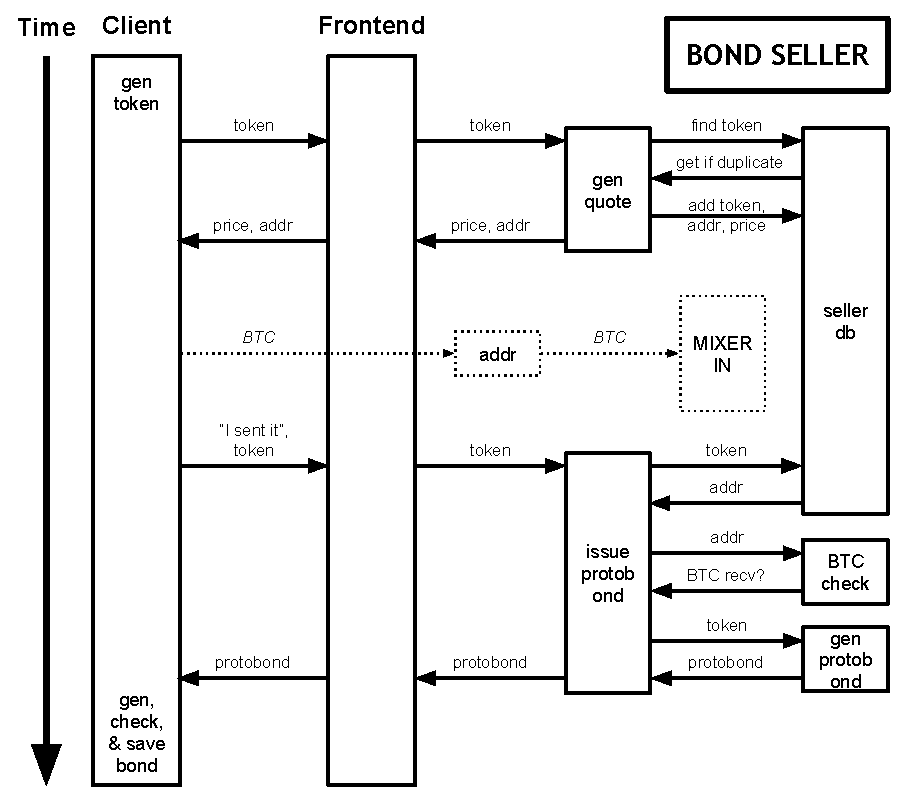
\includegraphics[width=14cm]{dryer21-bond-seller-diagram.pdf}
\end{center}
\caption{The seller privilege separation.\label{seller}}
\end{figure}
\begin{figure}[ht]
\begin{center}
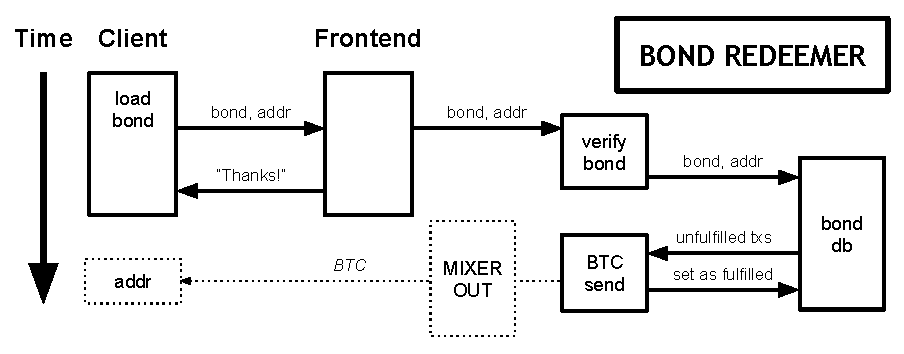
\includegraphics[width=14cm]{dryer21-bond-redeemer-diagram.pdf}
\end{center}
\caption{The redeemer privilege separation.\label{seller}}
\end{figure}

\end{document}

%% TODO: Should we include this section?
% If so, remove the \end{document} line above.

\end{document}
